%!TEX root = ../report.tex
\documentclass[report.tex]{subfiles}
\begin{document}
    \chapter{Related Works}

    % Divide the sections into Early, Late, Mid/Feature and Tightly-Coupled fusion methods
    \section{Adverse Weather Conditions Influence on Sensors}

    \begin{itemize}

        \item In the realm of autonomous robots, particularly self-driving vehicles and autonomous drones, object detection has emerged as a critical computer vision problem. These applications demand accurate 2D or 3D bounding boxes for objects in complex real-world scenarios, which often include cluttered scenes, unpredictable lighting, and adverse weather conditions. To address these challenges, the most promising autonomous vehicle systems rely on input from redundant sensor modalities, as documented by several recent studies \cite{caesar2020nuscenes, Sun_2020_CVPR, ziegler2014making}. These sensor modalities include cameras, LiDAR, radar, and emerging sensors like far-infrared (FIR) and near-infrared (NIR) sensors, which hold great potential for enabling reliable object detection in adverse environments \cite{bijelic2020seeing}.

        \item For a typical perception system, the most common sensor is camera, and it's actually the one element that is absolutely not replaceable in autonomous driving systems. But it's also one of the most vulnerable sensors to adverse weather conditions. A camera in rain, regardless of however high resolution, can be easily incapacitated by a single water drop on the emitter or lens \cite{mardirosian2021LiDAR} as shown in the Figure \ref{fig:camera_in_rain}. Heavy snow or hail could fluctuate the image intensity and obscure the edges of the pattern of a certain object in the image or video which leads to detection failure \cite{zang2019impact}. A particular weather phenomenon, strong light, directly from the sun or artificial light source like light pollution from a skyscraper may also cause severe trouble to cameras \cite{acarballo2020libre}.
            \begin{figure}[h]
                    \centering
                    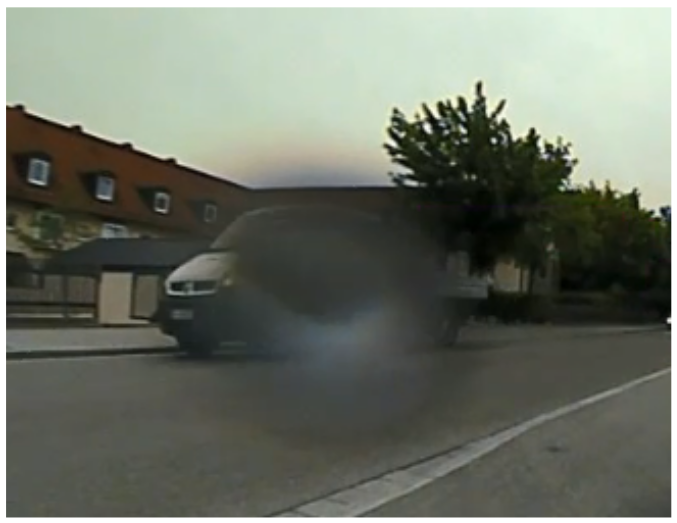
\includegraphics[width=0.5\textwidth]{images/rain_droplet.png}
                    \caption{Van occluded by a water droplet on the lens \cite{Nobis2020May}}
                    \label{fig:camera_in_rain}
            \end{figure}

        \item LiDAR is the second most commonly used sensor in autonomous driving systems. Fersch et al. \cite{fersch2016influence} suggest that for moderate levels of rainfall, LiDAR sensors with small apertures are not significantly affected. However, heavy and non-uniform precipitation rates can create clusters of fog that can lead to erroneous obstacle detection by the LiDARs. Hasirlioglu et al. \cite{hasirlioglu2016modeling} demonstrated that a rainfall rate exceeding 40 mm/hr leads to a significant drop in signal reflection intensity. Dense fog and smoke, as well as strong light, can also affect LiDAR sensors in adverse conditions \cite{Zhang2021Dec} \cite{acarballo2020libre}. Figure \ref{fig:lidar} shows an example of LiDAR performance in fog conditions where it creates small false obstacle clouds.
            \begin{figure}[h]
                    \centering
                    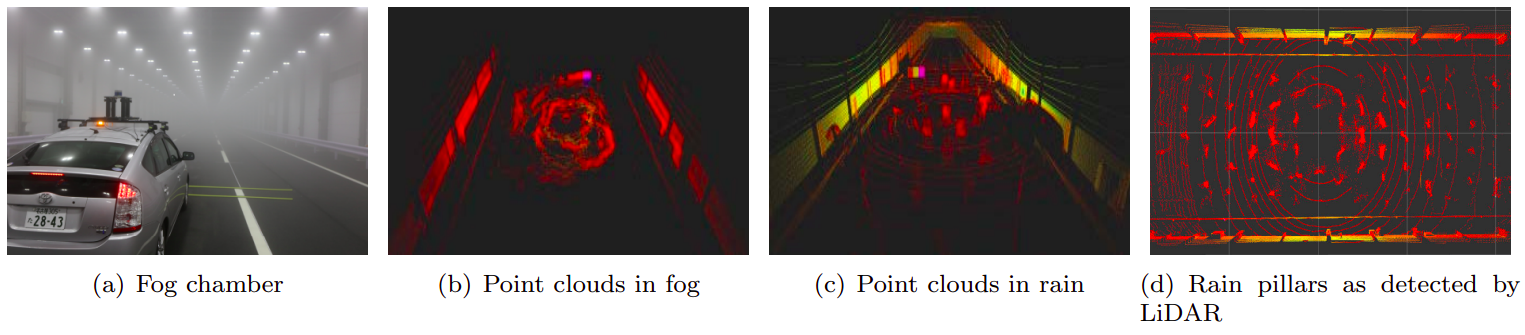
\includegraphics[width=0.9\textwidth]{images/lidar_issues.png}
                    \caption{LiDAR performance test \cite{Zhang2021Dec}}
                    \label{fig:lidar}
            \end{figure}

        \item Radar is the third most crucial sensor in autonomous driving systems and is widely used in mass-produced cars for active safety functions, such as automatic emergency braking (AEB) and forward collision warning (FCW). However, its significance is often overlooked from the perspective of perception tasks in autonomous driving. Unlike RGB cameras that use visible light bands (384$\sim$769 THz) and LiDARs that use infrared bands (361$\sim$331 THz), Radars use relatively longer wavelength radio bands (77$\sim$81 GHz), resulting in robust measurements in adverse weathers \cite{Paek2022Jun}. As reported by Ijaz et al. \cite{ijaz2012analysis} and Ismail \cite{gultepe2008measurements}, radar exhibits lower attenuation in rainy conditions than LiDAR. The attenuation of radar at 77 GHz is approximately 3.5 times lower (10 dB/km) than that of LiDAR at 905 nm (35 dB/km), demonstrating better robustness. Multiple experiments \cite{adams2012robotic, brooker2007seeing, xu2022learned, gourova2017analysis, zang2019impact} have revealed that attenuation and backscattering under dust, fog, snow, and light rain are negligible for radar, while its performance degrades under heavy rainfall. However, one of the significant drawbacks of radar is its low resolution, which makes it difficult to use in perception tasks. The radar point cloud is much sparser than LiDAR, limiting its usability. Recently, the next generation of 4D radar has emerged, which can provide denser points compared to conventional radar sensors.
            \begin{figure}[h]
                  \centering
                  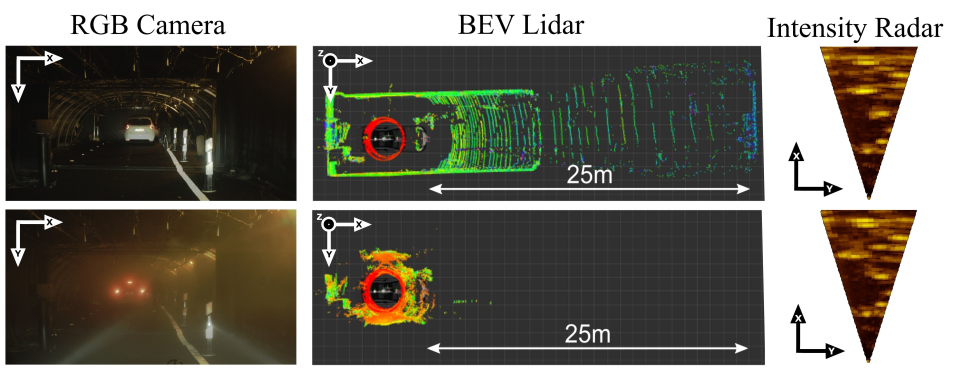
\includegraphics[width=0.8\textwidth]{images/lidar_in_fog.png}
                  \caption{\centering 1st row: clear weather condition, 2nd row: with fog. Shows that lidar affects by the fog but radar intensity remains the same \cite{bijelic2020seeing}}
                  \label{fig:lidar_in_fog}
            \end{figure}


        % ===> Why do we need multimodal perception?
        \item By now, it’s almost well established that the LiDAR or Camera architecture alone is not going to navigate through adverse weather conditions with enough safety assurance. But two forces combining together would be a different story with the additional strength. The same can be seen as discussed before from the Figure \ref{fig:sensors_intro_1} and \ref{fig:sensors_intro_2}. As a result, groups from all over the world come up with their own permutation and combination with camera, LiDAR, radar, infrared camera, gated camera, stereo camera, weather stations and other weather-related sensors.
        
    \end{itemize}

    \section{Multimodal Sensor Fusion}

    \begin{itemize}
        
        \item Radecki et al. \cite{radecki2016all} conducted a comprehensive review, investigating the efficacy of various sensors in a range of weather conditions including wet conditions, day and night, cloudy skies, glare, and dust. They engineered a robust system capable of tracking and classifying objects through a real-time, joint probabilistic perception algorithm. This advanced algorithm employs a dynamic selection of sensor subsets that are particularly suited to the prevailing weather conditions. The system not only elevates the general lower bound of perception ability but also optimizes its robustness and reliability through intelligent weighting of sensors and precise quantification of parameters based on the specific weather context. Such a design emphasizes the crucial role of real-time strategy shifts and intelligent sensor subset selection in maximizing the accuracy and reliability of multimodal perception systems.
        % 2016
        \item Limitations of Radecki et al.'s \cite{radecki2016all} study include an emphasis on optimal weather conditions and a lack of investigation into heavy traffic or urban areas, as well as deep learning-based fusion techniques. Future research should consider these limitations and explore the use of proposed Similarly-based methods for object detection in adverse weather datasets.
        
        \item FLIR System Inc. \cite{fused_aeb} and VSI Labs \cite{VSILabs} conducted a test on the first ever fused automated emergency braking (AEB) sensor suite in 2019, consisting of a thermal long-wave infrared (LWIR) camera, a radar, and a visible camera. The LWIR camera captures wavelengths ranging from 8 µm to 14 µm and operates under ambient temperature, known as the uncooled thermal camera. The sensor suite was evaluated alongside several cars equipped with AEB systems employing radar and visible cameras under various conditions including day-time, nighttime, and tunnel exit into sun glare. The comparison results indicate that while most AEB systems perform adequately during the day, the standard AEB almost collided with every mannequin under adverse conditions, whereas the LWIR sensor suite avoided any collision. This study underscores the potential of fusing camera and radar in challenging weather situations.
        % 2019
        \item The work done by FLIR System Inc. \cite{fused_aeb} and the VSI Labs \cite{VSILabs} by using a thermal camera for fusion as one of the sensors, which raises the concerns of the durability of such temperature-sensitive devices in real environments. This needs further validation in real environments in the future to ensure their usefulness in adverse weather conditions \cite{zang2019impact}.
        
        \item To address the problem of when to fuse the data in the neural network architecture, Nobis et al. \cite{nobis2019deep} proposed a CameraRadarFusionNet (CRF-Net), which was inspired from camera-LiDAR fusion \cite{yu2019multi} and \cite{caltagirone2019lidar}, to learn at which level the fusion of the sensor data was the most beneficial for the detection task. They used nuScenes \cite{caesar2020nuscenes} dataset and released their own TUM dataset. Furthermore, they introduced a new training strategy to focus the learning on a specific sensor type, which was called BlackIn. For feature fusion, the element-wise addition was adopted as the fusion operation. Their fusion method outperformed the image-only network on both datasets, which again shows the importance of fusing radar data into the detection task.
        % 2019
        \item Nobis et al. \cite{nobis2019deep} proposed the CameraRadarFusionNet (CRF-Net) to learn the optimal level for sensor data fusion in the neural network architecture for detection tasks. While their fusion method outperformed the image-only network on nuScenes \cite{caesar2020nuscenes} and their own TUM dataset, the improvement in detection performance was limited. The element-wise addition used for feature fusion was a simple method, and the baseline image network's performance was only slightly lower than the CRF-Net's performance. Additionally, the study did not provide an RGB sensor ablation study, so it was unclear whether their system was robust in the case of camera failure. According to Safa et al. \cite{safa2021fail}, the performance could be further improved by pre-processing the radar data before fusion.
        
        \item Yang et al. \cite{yang2020radarnet} proposed RadarNet for object detection and velocity estimation, that leverages radar and LiDAR sensors for perception. RadarNet employs early fusion to learn joint representations from both sensors and late fusion to incorporate the radial velocity evidence of radar and enhance the estimated object velocity. The authors evaluated their approach on the nuScenes dataset \cite{caesar2020nuscenes}.
        \item In the RadarNet architecture, proposed by Yang et al. \cite{yang2020radarnet}, the radar sensor data used from the nuScenes dataset, which has a very low resolution and hence it's not a good choice for studying the role of radar in perception. Object detection using radars is limited by low resolution and erroneous elevation estimates \cite{ulrich2021deepreflecs} \cite{drews2022deepfusion}. Therefore, one possible improvement is to include the radar sensor used in K-Radar dataset, which is a 4D radar with elevation angle of 30 degrees compare to 1 or 2 degrees for conventional radars, can be used to improve the performance of the RadarNet architecture.
        
        \item Bijelic et al. \cite{bijelic2020seeing} from Mercedes-Benz AG conducted a study on improving detection performance in adverse weather conditions using a deep multimodal sensor fusion approach. The authors equipped their test vehicle with various sensors, including stereo RGB cameras, a NIR camera, a 77 GHz radar, two LiDARs, an FIR camera, a weather station, and a road-friction sensor. They proposed an entropy-steered fusion approach where regions with low entropy were attenuated while entropy-rich regions were amplified during feature extraction. The exteroceptive sensor data were concatenated and trained using clear weather data, demonstrating strong adaptation to unseen adverse weather data. The fusion network was designed to generalize across different scenarios, and all the sensor data were projected into the camera coordinate system to ensure consistency. The fused detection performance outperformed LiDAR or image-only approaches under fog conditions.
            % \item TODO: add images
            \begin{figure}[h]
                \centering
                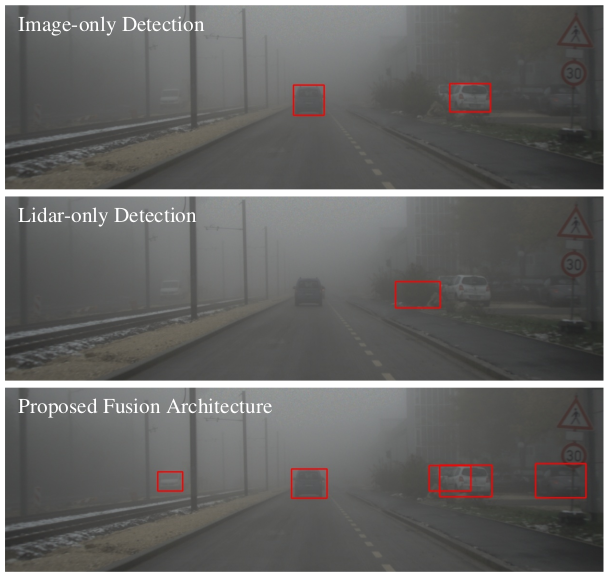
\includegraphics[width=0.4\textwidth]{images/seeing_through_fog.png}
                \caption{Highlighting the significance of fusing multimodal sensor data \cite{bijelic2020seeing}}
                \label{fig:seeing_through_fog}
            \end{figure}
        \item Bijelic et al. \cite{bijelic2020seeing} also provided the SeeingThroughFog or DENSE dataset for further research on multimodal sensor fusion in adverse weather conditions. This dataset comprises 10,000 km of driving data in Northern Europe, recorded during February and December 2019, under varying weather and illumination conditions. The dataset includes annotations for 5.5 k clear weather frames, 1 k dense fog frames, 1 k light fog frames, and 4 k frames captured in snow/rain.
        % 2020
        \item The study conducted by Bijelic et al. \cite{bijelic2020seeing} presents a multimodal sensor fusion approach that outperforms LiDAR or image-only approaches under fog conditions. However, one issue is that some essential radar information may be lost during the projection transformation used by the proposed method, leading to a loss of spatial information. Additionally, the large number of sensors required by the approach exceeds the typical expectations for an autonomous driving system, making it challenging to implement in real-world scenarios. The response and reaction time of the algorithm may also become a concern due to the bulk amount of data from multiple sensors. While the study demonstrated strong adaptation to adverse weather data, the performance of the radar used was limited by its low azimuth and elevation resolution \cite{Zhang2021Dec}. To address these limitations, future work could focus on improving the network architecture by using a higher resolution radar and using a transformer-based approaches to improve the performance of the sensor fusion approach in adverse weather conditions.
        
        % 2021
        \item Liu et al. \cite{liu2021robust} presented a novel approach to enhance the target recognition and tracking by fusing radar and camera data. In this approach, radar is considered as the primary sensor, and camera data is used as secondary information to complement the radar measurements. The authors evaluated the performance of their approach in challenging weather conditions, including rain and fog, as well as low visibility scenarios during nighttime. The experimental results revealed that radar-based detection exhibited high accuracy in detecting moving targets in wet weather, while the camera was more effective in target classification. Furthermore, the fusion of radar and camera data showed superior performance compared to LiDAR-based detection methods by over 33\%.
        
        % 2021
        \item Qian et al. \cite{qian2021robust} introduced a Multimodal Vehicle Detection Network (MVDNet) featuring LiDAR and radar. In the network architecture, MVDNet has a two-stage attention block in the fusion module. It first applied self-attention to each modality to extract features and then mixed them with region-wise features through cross attentions. Experiments showed that the fusion mechanism performs robustly in foggy weather. The authors trained and evaluated the model performance on SeeingThroughFog \cite{bijelic2020seeing} and the Oxford Radar Robotcar \cite{barnes2020oxford} datasets. And the evaluation shows much better performance than LiDAR alone in fog conditions.
        % 2021
        \item Qian et al. \cite{qian2021robust} proposed a Multimodal Vehicle Detection Network (MVDNet) that combines LiDAR and radar data using a two-stage attention block in the fusion module. Despite demonstrating robust performance in foggy weather conditions, the study has some limitations. Firstly, the misalignment between the LiDAR and radar data in the dataset is not corrected, which can affect the MVDNet's performance. Secondly, the simple label assignment strategy used in the loss computation procedure and the region-of-interest (ROI) assisted fusion design limits the model's performance. These factors suggest that there is room for improvement in the model's design, which could potentially be addressed by more advanced fusion techniques and better label assignment strategies \cite{yang2022ralibev}.
        
        \item Rawashdeh et al. \cite{rawashdeh2021drivable} developed a CNN-based sensor fusion approach for detecting drivable paths using cameras, LiDAR, and radar, which was evaluated using the DENSE dataset \cite{bijelic2020seeing}. Their multi-stream encoder-decoder network was designed to compensate for the asymmetric degradation of the input sensors at the highest level. The depth and number of blocks for each sensor in the architecture were determined by their respective input data densities, with the camera having the highest density, followed by LiDAR, and radar having the lowest. The fully connected network's outputs were reshaped into a 2-D array that was input to the decoder. The researchers showed that their model could effectively disregard road lines and edges that might otherwise cause false interpretations and accurately delineate the general drivable area.
        \item Rawashdeh et al. \cite{rawashdeh2021drivable} proposed a multimodal fusion approach for drivable path detection in poor weather conditions. However, the proposed method lacks a comparison with other state-of-the-art methods and does not investigate the real-time processing requirements and computational cost of the proposed algorithm, which could limit its practical applicability \cite{rawashdeh2021drivable}.
        
        % My chosen method 1, SAF-FCOS
        \item The paper by Chang et al. \cite{chang2020spatial} introduces a novel method for enhancing obstacle detection in autonomous driving systems. This method, called spatial attention fusion (SAF), effectively integrates data from millimeter-wave (mmWave) radar and camera sensors. SAF addresses the sparsity of radar points by generating an attention weight matrix that distinctively fuses vision features, diverging from traditional concatenation or element-wise addition fusion methods. This method can be integrated into the feature-extraction stage of existing deep learning object detection frameworks, facilitating end-to-end training. Additionally, the paper presents a generation model that converts radar points into images for neural network training. This type of image projection called radar imagery. The paper's findings indicate that this fusion approach significantly improves performance on nuScenes \cite{caesar2020nuscenes} dataset.
        
        % My chosen method 2, HRFuser
        \item Another work by Broedermann et al. \cite{broedermann2022hrfuser} presents an extended work on HRNet \cite{wang2020deep} and HRFormer \cite{yuan2021hrformer} to integrate multimodal sensors into a single network. It introduces HRFuser, a versatile, multi-resolution, multi-sensor fusion architecture that can efficiently integrate an arbitrary number of sensors like lidar, radar, and gated cameras, alongside standard cameras. HRFuser is built on the HRNet and HRFormer paradigms, preserving high-resolution representations and incorporating a novel multi-window cross-attention (MWCA) block for effective fusion across multiple resolutions. The system's generic design allows for easy scalability with various sensors without the need for specialized components for each sensor. Extensive testing on major autonomous driving datasets, including nuScenes \cite{caesar2020nuscenes}, and SeeingThroughFog \cite{bijelic2020seeing}, demonstrates HRFuser's superior performance over existing camera-only networks and sensor fusion methods, proving its efficacy in both standard and adverse weather conditions. HRFuser's adaptability to different sensor sets and its ability to selectively focus on relevant features from high-resolution data of additional sensors mark a significant advancement in the field of 2D object detection.
        
        % My chosen method 3, MT-DETR
        \item Recent work by Chu et al. \cite{chu2023mt} proposes a novel end-to-end multimodal multistage object detection network called MT-DETR (MulTi-sensor MulTimodal DTtection TRansformer) that leverages data from multiple sensors - camera, lidar, radar and time - to achieve robust detection, especially in adverse weather conditions. Here time modality is an additional binary image input to inform model about day or night. It employs specialized fusion modules - Residual Fusion Module (RFM) and Confidence Fusion Module (CFM) for hierarchical cross-modal feature fusion. The network also uses a Residual Enhancement Module (REM) to strengthen individual sensor branches. A multi-stage loss function further regularizes feature learning across modalities. Extensive experiments on the publicly available SeeingThroughFog \cite{bijelic2020seeing} dataset demonstrate that MT-DETR significantly outperforms existing unimodal and multimodal detection methods. Notably, when additionally trained on realistic synthetic foggy data generated by a novel camera-lidar synthesis algorithm, the performance boost is even higher.
        
        TODO: write about my choosen methods limitations
        
        \item Since most of the advance multimodal sensor fusion techniques, including state-of-the-art ones, are developed on clear weather datasets without paying special attention to the adverse weather conditions. And many of them use LiDAR and camera \cite{feng2020deep} as the primary sensors. This could be because of the availability of the datasets. Hence, there is a need to study the performance of these advance deep learning techniques in adverse weather conditions with the combination of other sensors like radar, thermal camera, infrared camera, etc.
      
        \item Currently, there is no general guideline available for the design of network architecture in multimodal sensor fusion, and several questions remain unanswered. According to Feng et al. \cite{feng2020deep}, these include 
        \begin{itemize}
              \item "what to fuse," such as LiDAR, radar, color camera, thermal camera, event camera, or ultrasonic sensors; 
              \item "how to fuse," which can include addition or mean, concatenation, ensemble methods, or mixture of experts; 
              \item "when to fuse," which can involve early, mid, late, or a combination of all fusion methods.
        \end{itemize}
  
        \item The lack of comparison with alternative models or datasets is a limitation of previous studies on multimodal sensor fusion. Many studies have only shown results for their own baseline models and custom datasets, which limits the generalization of their findings.
        
        \item While recent multimodal datasets have released baseline models with simple fusion methods, the use of more advanced fusion methods, such as transformer-based or tightly-coupled fusion, has the potential to improve their performance.
  
        \item Temporal information is a crucial aspect of sensor fusion, but very few multimodal fusion algorithms have been developed to handle this type of data \cite{bijelic2020seeing}. Although this project does not consider the temporal information in the fusion process, it is still a promising area for future research.
  
        \item There is a dearth of work in the literature utilizing 4D imaging radar sensor especially for adverse weather conditions, which is a promising area for future research. \cite{Zhou2022May}

    \end{itemize}

    TODO: try to accomodate these two sections in the above section
    
    \section{Synthetic Data for Adverse Weather Conditions}
    \begin{itemize}
        \item There are studies out there that use de-hazing techniques to remove the bad effects from adverse weather. While physical priors were previously used \cite{tan2008visibility, tarel2009fast}, data-driven methods using deep learning have been introduced. However, deep de-hazing models have high computational complexity and are unsuitable for ultra-high-definition images. Chen et al. \cite{chen2021psd} found that models trained on synthetic images do not generalize well to real-world hazy images, while Zhang et al. \cite{zhang2021learning} used temporal redundancy to perform video de-hazing and collected a dataset of real-world hazy and haze-free videos. Although collecting pairs of hazy and haze-free ground-truth images is challenging, professional haze/fog generators exist to simulate real-world conditions \cite{musat2021multi, timofte2018ntire}.
        \item Few researchers \cite{sun2021multi} \cite{zheng2020forkgan} \cite{lee2022perception} have also explored synthetic data generation for adverse weather conditions using GAN-based techniques from clean weather dataset eg. KITTI \cite{geiger2012we}, Cityscapes \cite{cordts2016cityscapes}, etc. However, the current methods are predominantly assessed on artificially created fog or rain images, along with a limited number of actual images under specific fog or rain models. Consequently, the capability of these algorithms to perform effectively under various adverse weather conditions and how their progress can be assessed in real-world scenarios remain unclear \cite{hassaballah2020vehicle}.
    \end{itemize}

    \section{Simulation}
    \begin{itemize}
        \item The emergence of autonomous driving, particularly in harsh weather conditions, has benefited greatly from simulation platforms and experimental facilities such as fog chambers or test roads. CARLA simulator \cite{dosovitskiy2017carla} is a popular virtual platform that allows researchers to create complex road environments and non-ego participants in infinite scenarios, which would be difficult and costly to replicate in real-world experiments. Furthermore, weather conditions, especially season-related or extreme climates-related, may not always be available for testing purposes. For instance, tropical regions cannot conduct snow tests, and natural rain showers may not last long enough to collect adequate experimental data. Most importantly, adverse weather conditions pose a danger to driving, and real-world tests always carry the risk of safety hazards, while simulators can provide an environment with zero risks \cite{Zhang2021Dec}.
    \end{itemize}
    % Dont know where to put DATASET related content
    % One entire section could be my comparative study on multimodal dataset
    \section{Available Dataset}
    TODO: remove this from here
    \begin{itemize}
        \item The majority of deep multimodal perception approaches rely on supervised learning, and therefore necessitate multimodal datasets with labeled ground truth for training deep neural networks. While several multimodal datasets are available, many of these datasets are collected under clear weather conditions or do not include all sensors, such as cameras, LiDAR, and radar. Unfortunately, the availability of multimodal datasets collected under adverse weather conditions with all three sensors is limited. Table 1 summarizes some of the available multimodal datasets for evaluating the performance of deep multimodal perception techniques in adverse weather conditions. Of these datasets, only the recently released K-Radar \cite{Paek2022Jun} incorporates a high-resolution 4D-radar sensor. In the table, C-R-L-N-F denotes the Camera, Radar, LiDAR, Near-infrared, and Far-infrared sensors, respectively.
            \begin{table}[h]
                \centering
                \caption{List multimodal datasets with adverse weather conditions}
                \label{tab:my-table}
                \begin{tabular}{|l|l|l|l|}
                    \hline
                    \textbf{Name}       & \textbf{Sensors} & \textbf{Reference}               & \textbf{Year} \\ \hline
                    DENSE               & CRLNF            & \cite{bijelic2020seeing}    & 2020          \\ \hline
                    EU Long-term        & CRL              & \cite{yan2020eu}            & 2020          \\ \hline
                    nuScenes            & CRL              & \cite{caesar2020nuscenes}   & 2020          \\ \hline
                    The Oxford RobotCar & CRL              & \cite{barnes2020oxford}     & 2020          \\ \hline
                    RADIATE             & CRL              & \cite{sheeny2021radiate}    & 2021          \\ \hline
                    K-Radar             & CRL              & \cite{Paek2022Jun}          & 2022          \\ \hline
                    aiMotive            & CRL              & \cite{matuszka2022aimotive} & 2022          \\ \hline
                    Boreas              & CRL              & \cite{burnett2022boreas}    & 2022          \\ \hline
                    WADS                & CRLNF            & \cite{kurup2022winter}      & 2023          \\ \hline
                \end{tabular}
            \end{table}

            \begin{figure}[h]
                \centering
                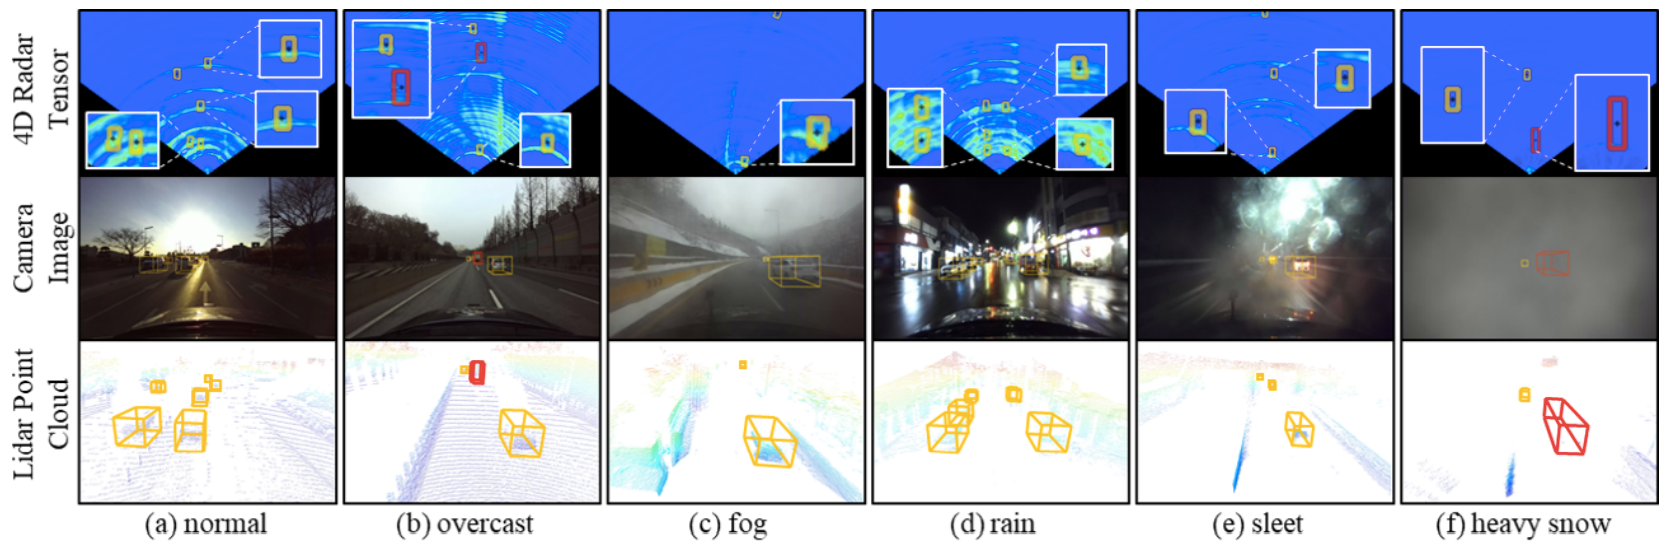
\includegraphics[width=1.0\textwidth]{images/all_sensors_in_adverse_weather.png}
                \caption{\centering Samples of K-Radar datasets for various weather conditions \cite{Paek2022Jun}}
                \label{fig:all_sensors_in_adverse_weather}
            \end{figure}
        \end{itemize}

\end{document}
